% Options for packages loaded elsewhere
\PassOptionsToPackage{unicode}{hyperref}
\PassOptionsToPackage{hyphens}{url}
%
\documentclass[
  ignorenonframetext,
]{beamer}
\usepackage{pgfpages}
\setbeamertemplate{caption}[numbered]
\setbeamertemplate{caption label separator}{: }
\setbeamercolor{caption name}{fg=normal text.fg}
\beamertemplatenavigationsymbolsempty
% Prevent slide breaks in the middle of a paragraph
\widowpenalties 1 10000
\raggedbottom
\setbeamertemplate{part page}{
  \centering
  \begin{beamercolorbox}[sep=16pt,center]{part title}
    \usebeamerfont{part title}\insertpart\par
  \end{beamercolorbox}
}
\setbeamertemplate{section page}{
  \centering
  \begin{beamercolorbox}[sep=12pt,center]{part title}
    \usebeamerfont{section title}\insertsection\par
  \end{beamercolorbox}
}
\setbeamertemplate{subsection page}{
  \centering
  \begin{beamercolorbox}[sep=8pt,center]{part title}
    \usebeamerfont{subsection title}\insertsubsection\par
  \end{beamercolorbox}
}
\AtBeginPart{
  \frame{\partpage}
}
\AtBeginSection{
  \ifbibliography
  \else
    \frame{\sectionpage}
  \fi
}
\AtBeginSubsection{
  \frame{\subsectionpage}
}
\usepackage{amsmath,amssymb}
\usepackage{iftex}
\ifPDFTeX
  \usepackage[T1]{fontenc}
  \usepackage[utf8]{inputenc}
  \usepackage{textcomp} % provide euro and other symbols
\else % if luatex or xetex
  \usepackage{unicode-math} % this also loads fontspec
  \defaultfontfeatures{Scale=MatchLowercase}
  \defaultfontfeatures[\rmfamily]{Ligatures=TeX,Scale=1}
\fi
\usepackage{lmodern}
\ifPDFTeX\else
  % xetex/luatex font selection
\fi
% Use upquote if available, for straight quotes in verbatim environments
\IfFileExists{upquote.sty}{\usepackage{upquote}}{}
\IfFileExists{microtype.sty}{% use microtype if available
  \usepackage[]{microtype}
  \UseMicrotypeSet[protrusion]{basicmath} % disable protrusion for tt fonts
}{}
\makeatletter
\@ifundefined{KOMAClassName}{% if non-KOMA class
  \IfFileExists{parskip.sty}{%
    \usepackage{parskip}
  }{% else
    \setlength{\parindent}{0pt}
    \setlength{\parskip}{6pt plus 2pt minus 1pt}}
}{% if KOMA class
  \KOMAoptions{parskip=half}}
\makeatother
\usepackage{xcolor}
\newif\ifbibliography
\usepackage{color}
\usepackage{fancyvrb}
\newcommand{\VerbBar}{|}
\newcommand{\VERB}{\Verb[commandchars=\\\{\}]}
\DefineVerbatimEnvironment{Highlighting}{Verbatim}{commandchars=\\\{\}}
% Add ',fontsize=\small' for more characters per line
\usepackage{framed}
\definecolor{shadecolor}{RGB}{248,248,248}
\newenvironment{Shaded}{\begin{snugshade}}{\end{snugshade}}
\newcommand{\AlertTok}[1]{\textcolor[rgb]{0.94,0.16,0.16}{#1}}
\newcommand{\AnnotationTok}[1]{\textcolor[rgb]{0.56,0.35,0.01}{\textbf{\textit{#1}}}}
\newcommand{\AttributeTok}[1]{\textcolor[rgb]{0.13,0.29,0.53}{#1}}
\newcommand{\BaseNTok}[1]{\textcolor[rgb]{0.00,0.00,0.81}{#1}}
\newcommand{\BuiltInTok}[1]{#1}
\newcommand{\CharTok}[1]{\textcolor[rgb]{0.31,0.60,0.02}{#1}}
\newcommand{\CommentTok}[1]{\textcolor[rgb]{0.56,0.35,0.01}{\textit{#1}}}
\newcommand{\CommentVarTok}[1]{\textcolor[rgb]{0.56,0.35,0.01}{\textbf{\textit{#1}}}}
\newcommand{\ConstantTok}[1]{\textcolor[rgb]{0.56,0.35,0.01}{#1}}
\newcommand{\ControlFlowTok}[1]{\textcolor[rgb]{0.13,0.29,0.53}{\textbf{#1}}}
\newcommand{\DataTypeTok}[1]{\textcolor[rgb]{0.13,0.29,0.53}{#1}}
\newcommand{\DecValTok}[1]{\textcolor[rgb]{0.00,0.00,0.81}{#1}}
\newcommand{\DocumentationTok}[1]{\textcolor[rgb]{0.56,0.35,0.01}{\textbf{\textit{#1}}}}
\newcommand{\ErrorTok}[1]{\textcolor[rgb]{0.64,0.00,0.00}{\textbf{#1}}}
\newcommand{\ExtensionTok}[1]{#1}
\newcommand{\FloatTok}[1]{\textcolor[rgb]{0.00,0.00,0.81}{#1}}
\newcommand{\FunctionTok}[1]{\textcolor[rgb]{0.13,0.29,0.53}{\textbf{#1}}}
\newcommand{\ImportTok}[1]{#1}
\newcommand{\InformationTok}[1]{\textcolor[rgb]{0.56,0.35,0.01}{\textbf{\textit{#1}}}}
\newcommand{\KeywordTok}[1]{\textcolor[rgb]{0.13,0.29,0.53}{\textbf{#1}}}
\newcommand{\NormalTok}[1]{#1}
\newcommand{\OperatorTok}[1]{\textcolor[rgb]{0.81,0.36,0.00}{\textbf{#1}}}
\newcommand{\OtherTok}[1]{\textcolor[rgb]{0.56,0.35,0.01}{#1}}
\newcommand{\PreprocessorTok}[1]{\textcolor[rgb]{0.56,0.35,0.01}{\textit{#1}}}
\newcommand{\RegionMarkerTok}[1]{#1}
\newcommand{\SpecialCharTok}[1]{\textcolor[rgb]{0.81,0.36,0.00}{\textbf{#1}}}
\newcommand{\SpecialStringTok}[1]{\textcolor[rgb]{0.31,0.60,0.02}{#1}}
\newcommand{\StringTok}[1]{\textcolor[rgb]{0.31,0.60,0.02}{#1}}
\newcommand{\VariableTok}[1]{\textcolor[rgb]{0.00,0.00,0.00}{#1}}
\newcommand{\VerbatimStringTok}[1]{\textcolor[rgb]{0.31,0.60,0.02}{#1}}
\newcommand{\WarningTok}[1]{\textcolor[rgb]{0.56,0.35,0.01}{\textbf{\textit{#1}}}}
\setlength{\emergencystretch}{3em} % prevent overfull lines
\providecommand{\tightlist}{%
  \setlength{\itemsep}{0pt}\setlength{\parskip}{0pt}}
\setcounter{secnumdepth}{-\maxdimen} % remove section numbering
\usepackage{../../beamer_style/beamer_style}
\ifLuaTeX
  \usepackage{selnolig}  % disable illegal ligatures
\fi
\usepackage{bookmark}
\IfFileExists{xurl.sty}{\usepackage{xurl}}{} % add URL line breaks if available
\urlstyle{same}
\hypersetup{
  pdftitle={Intermediate  Programming},
  pdfauthor={Jake S. Truscott, Ph.D},
  hidelinks,
  pdfcreator={LaTeX via pandoc}}

\title{Intermediate \texttt{R} Programming}
\subtitle{POS6933: Computational Social Science}
\author{Jake S. Truscott, Ph.D}
\date{}
\institute{\vspace{-5mm}

University of Florida \newline Spring 2026 \newline \newline \newline

\includegraphics[width=3cm]{../../beamer_style/UF.png} \quad 

\includegraphics[width=3.1cm]{../../images/CSS_POLS_UF_Logo.png}}

\begin{document}
\frame{\titlepage}

\begin{frame}{Overview}
\phantomsection\label{overview}
\begin{itemize}
\tightlist
\item
  Random Number Generation in \texttt{R} \vspace{2.5mm}
\item
  Loops and Iteration \vspace{2.5mm}
\item
  Visualizing Data and Relationships Using \texttt{ggplot::()}
\end{itemize}
\end{frame}

\section{Random Number Generation}\label{random-number-generation}

\begin{frame}{Coin Flips}
\phantomsection\label{coin-flips}
\centering

\textbf{What is the probability that any independent coin flip will land on heads?}
\pause 

\par \vspace{5mm}

\textbf{Does this change if I flip 50 times?} \pause 

\par \vspace{5mm}

\textbf{What about 100 times?}\pause 

\par \vspace{5mm}

\textbf{What about 1000 times?}\pause 

\par \vspace{5mm}

\textbf{What about 10000 times?}
\end{frame}

\begin{frame}{Coin Flips (Cont.)}
\phantomsection\label{coin-flips-cont.}
\small

\begin{center}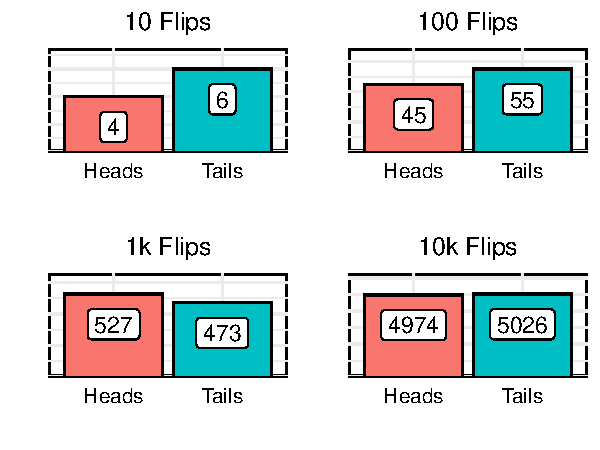
\includegraphics{Class_2_Intermediate_R_Programming_files/figure-beamer/coin_flips_sim-1} \end{center}
\end{frame}

\begin{frame}[fragile]{Coin Flips (Cont.)}
\phantomsection\label{coin-flips-cont.-1}
\begin{itemize}
\tightlist
\item
  We can use \texttt{sample()} to randomly select elements from a vector
\item
  In this case, a coin flip where \(p(heads) = p(tails) = 0.5\)
\end{itemize}

\begin{Shaded}
\begin{Highlighting}[]
\NormalTok{sides }\OtherTok{\textless{}{-}} \FunctionTok{c}\NormalTok{(}\StringTok{"Heads"}\NormalTok{, }\StringTok{"Tails"}\NormalTok{)  }\CommentTok{\# Flip Options}
\NormalTok{single\_flip }\OtherTok{\textless{}{-}} \FunctionTok{sample}\NormalTok{(sides, }\AttributeTok{size =} \DecValTok{1}\NormalTok{)  }\CommentTok{\# Single Draw}
\FunctionTok{print}\NormalTok{(single\_flip)}
\end{Highlighting}
\end{Shaded}

\begin{verbatim}
[1] "Heads"
\end{verbatim}
\end{frame}

\begin{frame}[fragile]{6-Sided Die}
\phantomsection\label{sided-die}
\begin{itemize}
\tightlist
\item
  We can use the same approach to ``roll'' a six-sided die.
\end{itemize}

\begin{Shaded}
\begin{Highlighting}[]
\NormalTok{sides }\OtherTok{\textless{}{-}} \FunctionTok{c}\NormalTok{(}\DecValTok{1}\SpecialCharTok{:}\DecValTok{6}\NormalTok{)  }\CommentTok{\# 1, 2, 3, 4, 5, 6}
\NormalTok{single\_roll }\OtherTok{\textless{}{-}} \FunctionTok{sample}\NormalTok{(sides, }\AttributeTok{size =} \DecValTok{1}\NormalTok{)  }\CommentTok{\# Single Roll}
\FunctionTok{message}\NormalTok{(}\StringTok{"Result of Single Roll: "}\NormalTok{, single\_roll)}
\end{Highlighting}
\end{Shaded}

\begin{verbatim}
Result of Single Roll: 1
\end{verbatim}
\end{frame}

\begin{frame}[fragile]{Poker Hands}
\phantomsection\label{poker-hands}
\begin{itemize}
\tightlist
\item
  We can even use it to do more complex operations like simulate a
  random draw from 5-card Poker \tiny
\end{itemize}

\begin{Shaded}
\begin{Highlighting}[]
\NormalTok{cards }\OtherTok{\textless{}{-}} \FunctionTok{as.character}\NormalTok{(}\FunctionTok{c}\NormalTok{(}\DecValTok{2}\SpecialCharTok{:}\DecValTok{10}\NormalTok{, }\StringTok{"J"}\NormalTok{, }\StringTok{"Q"}\NormalTok{, }\StringTok{"K"}\NormalTok{, }\StringTok{"A"}\NormalTok{))}
\CommentTok{\# All Card Values}
\NormalTok{suits }\OtherTok{\textless{}{-}} \FunctionTok{c}\NormalTok{(}\StringTok{"Hearts"}\NormalTok{, }\StringTok{"Diamonds"}\NormalTok{, }\StringTok{"Spades"}\NormalTok{, }\StringTok{"Clubs"}\NormalTok{)}
\CommentTok{\# Suits}

\NormalTok{deck }\OtherTok{\textless{}{-}} \FunctionTok{expand.grid}\NormalTok{(}\AttributeTok{value =}\NormalTok{ cards, }\AttributeTok{suit =}\NormalTok{ suits) }\SpecialCharTok{|\textgreater{}}
    \FunctionTok{mutate}\NormalTok{(}\AttributeTok{card =} \FunctionTok{paste}\NormalTok{(value, }\StringTok{"of"}\NormalTok{, suit)) }\SpecialCharTok{|\textgreater{}}
    \FunctionTok{pull}\NormalTok{(card)  }\CommentTok{\# Create a Full Deck}

\NormalTok{random\_draw }\OtherTok{\textless{}{-}} \FunctionTok{sample}\NormalTok{(deck, }\AttributeTok{size =} \DecValTok{5}\NormalTok{, }\AttributeTok{replace =}\NormalTok{ F)}
\CommentTok{\# Random 5{-}Card Draw w/out Replacement}
\end{Highlighting}
\end{Shaded}
\end{frame}

\begin{frame}[fragile]{Poker Hands (Cont.)}
\phantomsection\label{poker-hands-cont.}
\begin{verbatim}
Hand: 
9 of Clubs
Q of Clubs
6 of Clubs
2 of Diamonds
6 of Hearts
\end{verbatim}
\end{frame}

\begin{frame}{Generating Distributions}
\phantomsection\label{generating-distributions}
\begin{itemize}
\tightlist
\item
  What if we wanted to move beyond random selection where each draw or
  iteration exists with equal probability or within a uniform
  distribution?

  \par \vspace{5mm}
\item
  \texttt{R} is very flexible and capable of illustrating sampling
  distributions against expected outcomes
\end{itemize}
\end{frame}

\begin{frame}[fragile]{Generating Distributions (Standard Normal)}
\phantomsection\label{generating-distributions-standard-normal}
\begin{itemize}
\tightlist
\item
  Let's start with 1000 samples from a standard normal distribution
  where \(\mu\) = 50 and \(\sigma\) = 10
\end{itemize}

\begin{Shaded}
\begin{Highlighting}[]
\NormalTok{normal }\OtherTok{\textless{}{-}} \FunctionTok{rnorm}\NormalTok{(}\DecValTok{1000}\NormalTok{, }\AttributeTok{mean =} \DecValTok{50}\NormalTok{, }\AttributeTok{sd =} \DecValTok{10}\NormalTok{)}
\end{Highlighting}
\end{Shaded}

\begin{center}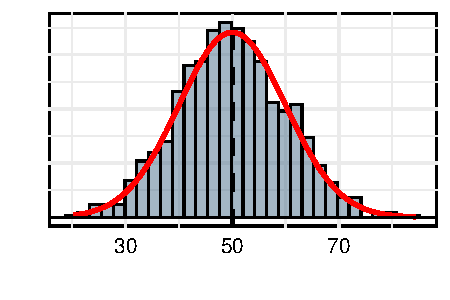
\includegraphics{Class_2_Intermediate_R_Programming_files/figure-beamer/normal_distribution_figure-1} \end{center}
\end{frame}

\begin{frame}{Generating Distributions (Standard Normal)}
\phantomsection\label{generating-distributions-standard-normal-1}
\begin{itemize}
\tightlist
\item
  \textbf{Your Turn}: Generate 1000 draws from a standard normal
  distribution where \(\mu\) = 25 and \(\sigma\) = 10.
\end{itemize}
\end{frame}

\end{document}
